\documentclass{article}
\usepackage[paperheight=1in,paperwidth=3in,top=0.1in,bottom=0.1in,right=0.1in,left=0.1in]{geometry}
\usepackage{tikz}
\usetikzlibrary{quantikz2}
\usepackage{physics}
\begin{document}


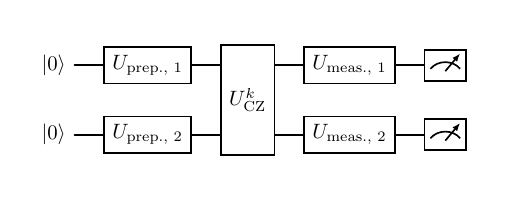
\begin{tikzpicture}
        \node[scale=0.75] {
        \begin{quantikz}
        \lstick{$\ket{0}$}& \gate{U_\text{prep., 1}}  & \gate[2]{U^k_{\text{CZ}}} & \gate{U_\text{meas., 1}} & \meter{}\\
        \lstick{$\ket{0}$}& \gate{U_\text{prep., 2}} & &  \gate{U_\text{meas., 2}} & \meter{}
        \end{quantikz} };
        \end{tikzpicture} 

\end{document}